\documentclass[tikz]{standalone}

\usepackage{amsmath}

\begin{document}
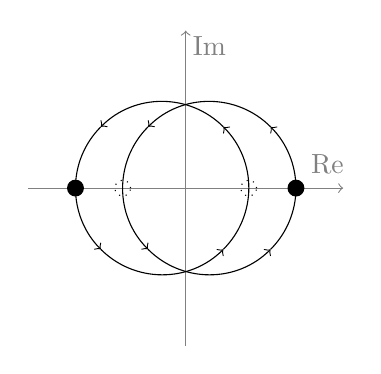
\begin{tikzpicture}

% Axes
\draw[->, gray] (+0, -2) -- (+0, +2);
\draw[->, gray] (-2, +0) -- (+2, +0);
\node[gray] at (+1.8, +0.3) {$\text{Re}$};
\node[gray] at (+0.3, +1.8) {$\text{Im}$};

% Initial points
\filldraw (-1.4, 0) circle (0.1);
\filldraw (+1.4, 0) circle (0.1);

% Midpoints
\draw[dotted] (+0.8, 0) circle (0.1);
\draw[dotted] (-0.8, 0) circle (0.1);

% Paths
\draw[->] (-1.400, +0.000) arc (180:225:1.1);
\draw[->] (-1.078, -0.778) arc (225:315:1.1);
\draw[->] (+0.478, -0.778) arc (-45:45:1.1);
\draw[->] (+0.478, +0.778) arc (45:135:1.1);
\draw (-1.078, +0.778) arc (135:180:1.1);
\draw[->] (+1.400, +0.000) arc (0:45:1.1);
\draw[->] (+1.078, +0.778) arc (45:135:1.1);
\draw[->] (-0.478, +0.778) arc (135:225:1.1);
\draw[->] (-0.478, -0.778) arc (225:315:1.1);
\draw (+1.078, -0.778) arc (315:360:1.1);

\end{tikzpicture}
\end{document}
